\subsection{Gas-phase chemistry}

Five kinetic mechanisms were chosen for comparison with the experimental data: FFCM2~\citep{ZDV2023}, Caltech~\citep{blanquart2009chemical}, CRECK~\citep{saggese2015kinetic}, KAUST~\citep{wang2013pah}, and ABF~\citep{appel2000kinetic}. We have provided a detailed comparison of the measured and predicted time histories of species using the same kinetic mechanisms elsewhere~\citep{clark2025}. Here, we focus on the temperature trends of major species, shown in Fig.~\ref{fig:interm_sampled_comp} (i) to identify the kinetic mechanism that most accurately describes the gas chemistry, and (ii) to highlight the connection between the temperature trends of CB yield and morphology with those of species. For $\mathrm{CH_4}$ (Fig.~\ref{fig:interm_sampled_comp}a), all mechanisms predict a nearly linear decrease with $\mathrm{T_5}$, consistent with the measurements, but a monotonic increase is observed for $\mathrm{C_2H_2}$ (Fig.~\ref{fig:interm_sampled_comp}c). FFCM2 providing the best agreement across the entire temperature range for both species, while Caltech also remains within the experimental uncertainty for $\mathrm{C_2H_2}$. In contrast, $\mathrm{C_2H_4}$ (Fig.~\ref{fig:interm_sampled_comp}b) shows a steep decline between $\mathrm{T_5}$$\approx$1900~K and 2100~K, followed by a more gradual decrease at higher temperatures. All mechanisms capture this trend, but large variability exists below $\mathrm{T_5}$$\approx$2100~K, especially between KAUST and FFCM2, while their predictions converge at higher temperatures. For A2R5 (Fig.\ref{fig:interm_sampled_comp}d), all mechanisms capture the bell-shape dependence of A2R5 with the peak $\mathrm{T_5}$$\approx$2203~K, whereas ABF slightly increasing with mole fractions less than $10^{-6}$ throughout. Based on the kinetic analysis, the Caltech mechanism is chosen for soot modelling because it provides a relatively accurate description of gas chemistry and also includes the designated soot precursors.
%Fig.\ref{fig:interm_timehis_comp} shows the measured and simulated time-history of the mole fraction of $\mathrm{CH_4}$, $\mathrm{C_2H_4}$, $\mathrm{C_2H_2}$, A2R5 for $\mathrm{T_5}=1984$~K and $\mathrm{T_5}=2203$~K as the representatives of the studied temperature range. The mole fraction of A2R5 was not measured experimentally. The mole fraction of species for all temperature conditions are presented in Figs.~\ref{fig:ch4_all}-\ref{fig:c2h2_all} in the supplementary material. The methane decompositon rate increases significantly with temperature.  The time at which $\mathrm{CH_4}$ mole fraction decays by 50\%, decreases from 0.4~ms at $\mathrm{T_5}=1984$~K to 0.06~ms at $\mathrm{T_5}=2203$~K. All mechanisms capture the overall trend, but CRECK and ABF noticeably overpredict and underpredict $\mathrm{CH_4}$ mole fraction at $\mathrm{T_5}=1984$~K with a relative error of 18\% and 31\%, respectively, after 1 ms of reaction time. The predictions of Caltech, KAUST and FFCM2 are within the uncertainty range of measurements ($\pm7.5\%$). At $\mathrm{T_5}=2203$~K (Fig.\ref{fig:interm_timehis_comp}b), Caltech~\citep{blanquart2009chemical} and KAUST also underpredict $\mathrm{CH_4}$ mole fraction similar to CRECK, but ABF and FFCM2 remain close to the upper and lower bounds of the uncertainty range, respectively,
% \begin{figure}[!t]
% 	\centering
% 	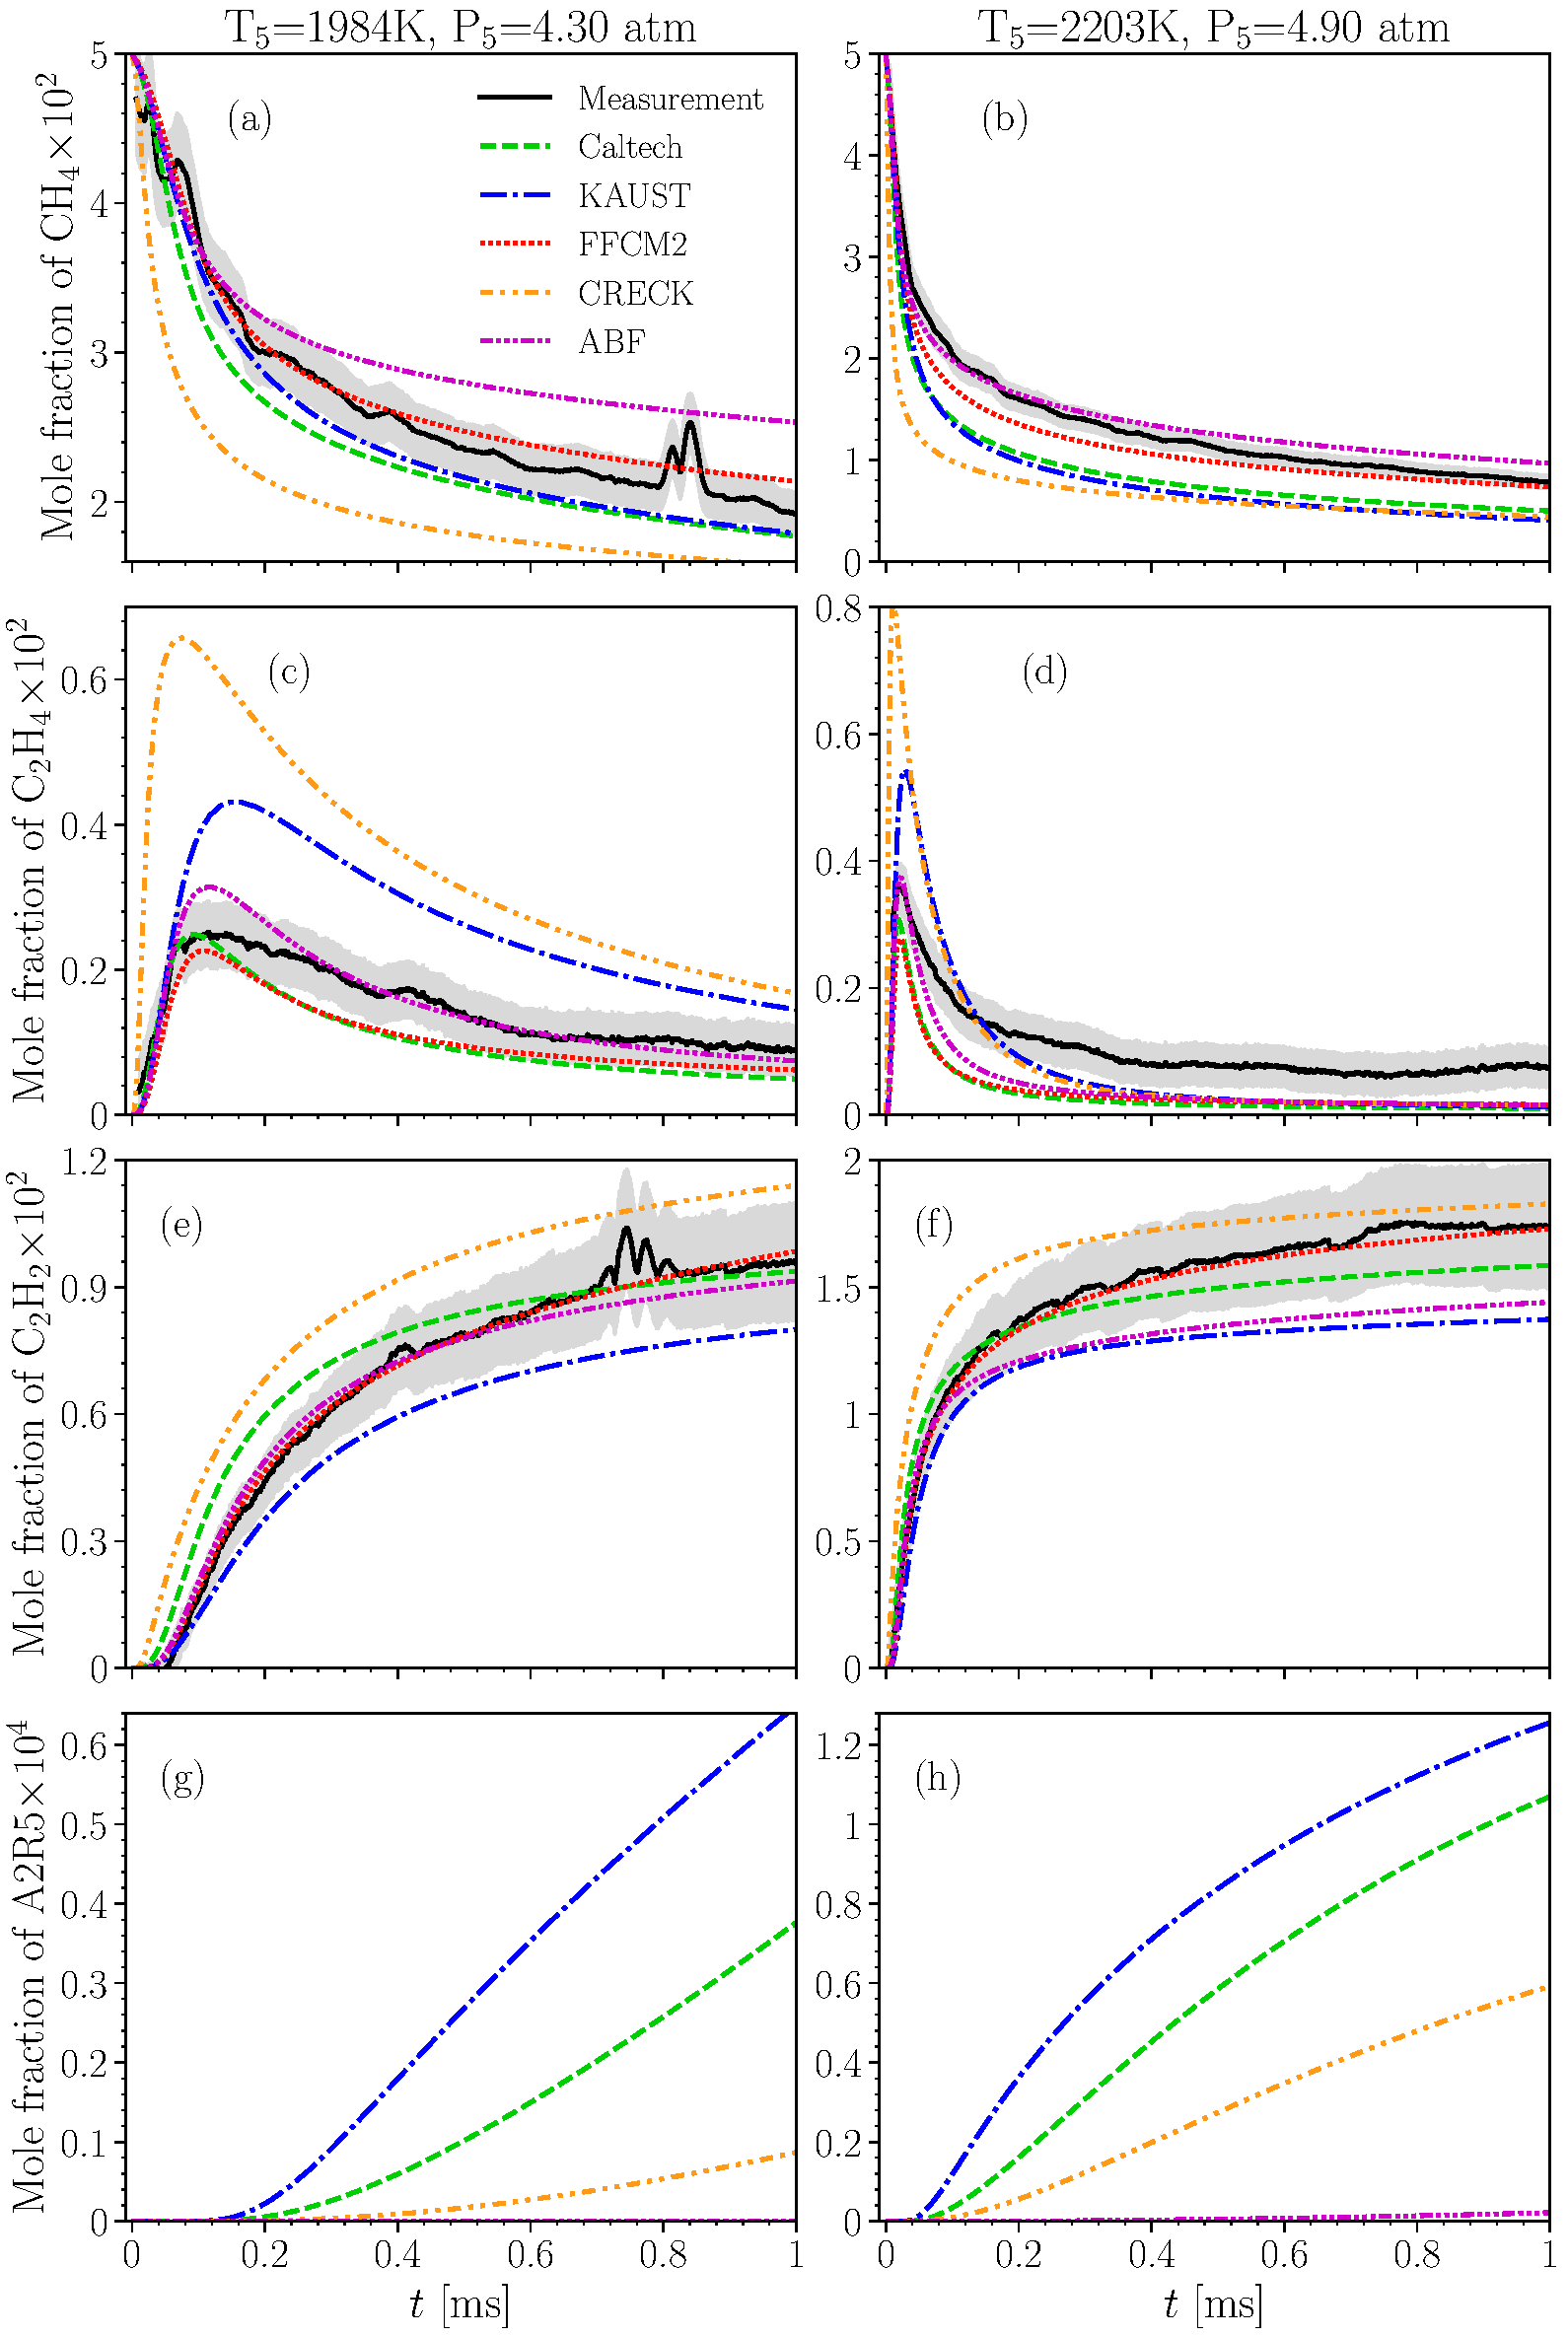
\includegraphics[width=0.47\textwidth]{Figures/CH4_C2H4_C2H2_A2R5_2conds.pdf}
% 	\caption{The mole fraction time-history measurements of $\mathrm{CH_4}$ (a, b), $\mathrm{C_2H_4}$ (c, d), and $\mathrm{C_2H_2}$ (e, f) compared with the predictions of different kinetic mechanisms for $\mathrm{T_5}=1984$~K and $\mathrm{T_5}=2203$~K. The mole fraction of A2R5 (g, h) is not available in the measurements and the FFCM2 mechanism. Shaded region around each measurement indicates experimental uncertainty.}
% 	\label{fig:interm_timehis_comp} 
% \end{figure}
% At $\mathrm{T_5}=1984$K, the mole fraction of $\mathrm{C_2H_4}$ rises rapidly within the first 0.12ms of decomposition, reaches a peak, and then gradually declines toward its final value. CRECK and KAUST significantly overpredict the peak $\mathrm{C_2H_4}$ mole fraction at both temperatures, whereas FFCM2, ABF, and Caltech provide predictions closer to the measurements. Beyond 0.2~ms, however, all mechanisms exhibit substantial underprediction relative to the experimental data toward the end of the simulation. Carbon flux analysis for all mechanisms identifies $\mathrm{C_2H_4}$ as a key precursor to $\mathrm{C_2H_2}$ formation through the vinyl radical ($\mathrm{C_2H_3}$) pathway.

% The performance of the mechanisms varies notably with temperature. While ABF reproduces the overall trend of $\mathrm{C_2H_2}$ mole fraction, it deviates significantly from the measurement uncertainty bounds. CRECK and KAUST exhibit consistent biases, with CRECK consistently underestimating and KAUST overestimating the measured values at both temperatures. Among the mechanisms, FFCM2 provides the best agreement with $\mathrm{C_2H_2}$ measurements across the entire range, whereas Caltech’s predictions remain within the uncertainty limits except for the early-time rise of $\mathrm{C_2H_2}$ ($\le 0.3$~ms) at $\mathrm{T_5}=1984$~K.

% All mechanisms predict an increasing trend for A2R5 mole fraction, but with substantial variability. Results from FFCM2 are omitted in Fig.~\ref{fig:interm_timehis_comp}g and h because this mechanism does not include PAH chemistry. The ABF mechanism predicts very low A2R5 mole fractions by 1~ms ($\le 10^{-6}$), whereas KAUST yields the highest values at both temperatures. Caltech predicts a higher A2R5 mole fraction than CRECK, which aligns with its lower $\mathrm{C_2H_2}$ mole fraction, suggesting that the Caltech mechanism converts more $\mathrm{C_2H_2}$ into PAHs.
% Fig.~\ref{fig:interm_sampled_comp} depicts the temperature dependence of species mole fractions sampled at 0.5~ms. For $\mathrm{CH_4}$ (Fig.~\ref{fig:interm_timehis_comp}a), all mechanisms predict a nearly linear decrease with $\mathrm{T_5}$, consistent with the measurements, but a monotonic increase is observed for $\mathrm{C_2H_2}$ (Fig.~\ref{fig:interm_sampled_comp}c). FFCM2 providing the best agreement across the entire temperature range for both species, while Caltech also remains within the experimental uncertainty for $\mathrm{C_2H_2}$. In contrast, $\mathrm{C_2H_4}$ (Fig.~\ref{fig:interm_sampled_comp}b) shows a steep decline between $\mathrm{T_5}$$\approx$1900~K and 2100~K, followed by a more gradual decrease at higher temperatures. All mechanisms capture this trend, but large variability exists below $\mathrm{T_5}$$\approx$2100~K, especially between KAUST and FFCM2, while their predictions converge at higher temperatures. For A2R5 (Fig.\ref{fig:interm_sampled_comp}d), all mechanisms capture the bell-shape dependence of A2R5 with the peak $\mathrm{T_5}$$\approx$2203~K, whereas ABF slightly increasing with mole fractions less than $10^{-6}$ throughout. Based on the kinetic analysis, the Caltech mechanism is chosen for soot modelling because it provides a relatively accurate description of gas chemistry and also includes the designated soot precursors.


\begin{figure}[!t]
	\centering
	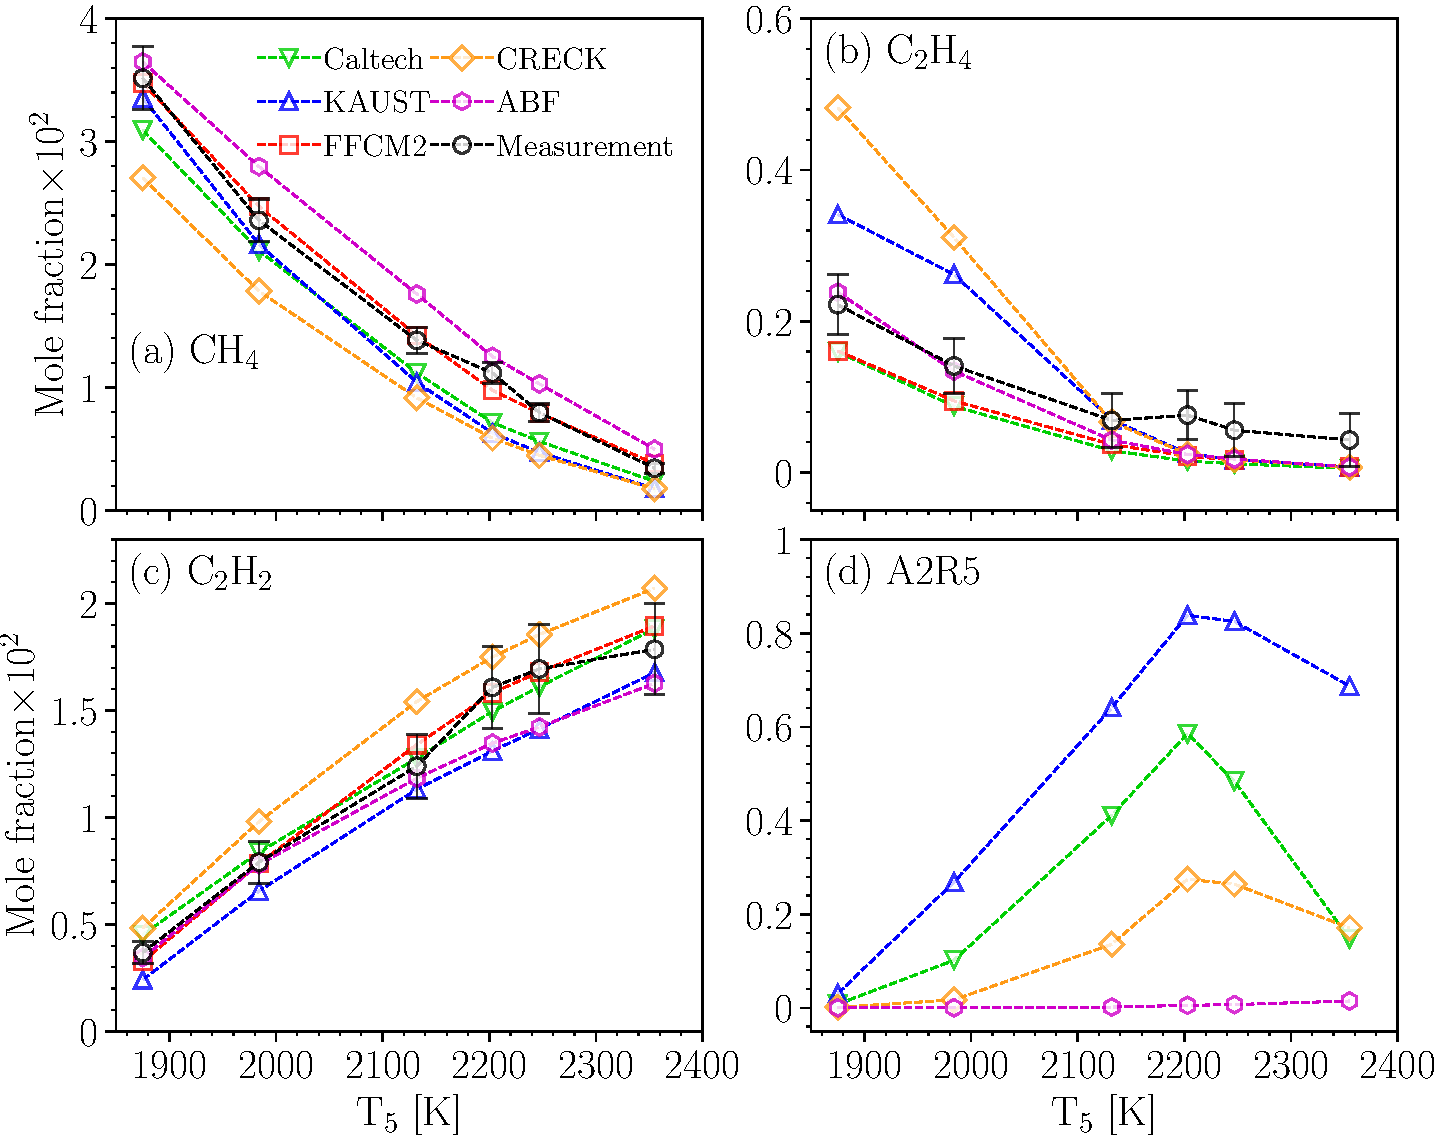
\includegraphics[width=0.49\textwidth]{Figures/CH4_C2H4_C2H2_A2R5_allconds_sampled.pdf}
	\caption{The mole fraction of $\mathrm{CH_4}$ (a), $\mathrm{C_2H_4}$ (b), and $\mathrm{C_2H_2}$ (c) at $t=0.5$~ms compared with the predictions of different kinetic mechanisms for $\mathrm{T_5}=1875$, 1984, 2132, 2203, 2247, 2355~K. Errors bars indicate experimental uncertainty of measurements, and the dashed line is added to show the trends.}
	\label{fig:interm_sampled_comp} 
\end{figure}



